\section{Einleitung}
Im Rahmen des Projektes Ausgewählte Themen der Automatisierungstechnik wurde ein modularer Drumcomputer entworfen.
Dieses Dokument enthält eine detaillierte Dokumentation der Montage des Drumcomputers, um den Nachbau zu ermöglichen.

\section{Gehäuse}
\subsection*{Aufbau des Eurorack Gehäuses}
Das Gehäuse wird auf einem gebrauchten Baugruppenträger aufgebaut.
Alternativ sind auch fertige Eurorackgehäuse am Markt erhältlich, sodass dieser Schritt nicht zwingend notwendig ist.

Da der Baugruppenträger an Ober- Unter und Rückseite offen ist, werden Gehäusebdeckungen gefertigt.
Ober- und Unterseite werden mit zwei 1 mm starken Edelstahlblechen abgedeckt.
Diese werden auf 426,5 mm x 128,5 mm zugeschnitten, zur Montage am Baugruppenträger werden an der Vorder- und Hinterkante drei 3 mm Bohrungen gesetzt. Mit M2,5x10 Zylinderkopfschrauben und passenden Muttern wurden die Bleche an der dafür vorgesehenen Bohrungen des Baugruppenträgers befestigt.

Da der Baugruppenträger deutliche Gebrauchsspuren hatte, wurden alle Metallteile lackiert.

Für die Rückseite des Gehäuses werden 4 Abdeckungen mit OpenSCAD entworfen mit dem 3D-Drucker gefertigt.
Diese sind im Verzeichnis \texttt{./3d/gehäuseabdeckungen} zu finden.
Eine der Abdeckungen ist mit einem Ausschnitt zur Montage einer Kaltgerätebuchse versehen.
Die Rückplatten lassen sich mit M2.5x14 Schrauben am Baugruppenträger befestigen.
Die Montage der Kaltgerätebuchse erfolgt mit M3x12 Blechschrauben.
An die Lötösen der Kaltgerätebuchse wurden drei $1,5\,\unit{mm^2}$ Kabel angelötet, die Lötstellen wurden mit Schrumpfschlauch abgedeckt.


\subsection*{Montage des Netzteils}
Als Netzteil wird ein Gerät des Herstellers Mean Well mit Modellnummer \enquote{mw rt-65b} montiert.
Dieses bietet die drei nötigen Betriebsspannungen $+12\,\unit{V}$, $-12\,\unit{V}$ und $+5\,\unit{V}$.

Die Montage erfolgt an der Innenseite der linken Seitenplatte des Baugruppenträgers mit einer M5 und einer M3 Schraube sowie passenden Muttern. Dazu müssen zwei Bohrungen gesetzt werden.

Das so vormontierte Gehäuse ist in Abbildung \ref{fig:baugruppentraeger} abgebildet
\begin{figure}[h]
    \centering
    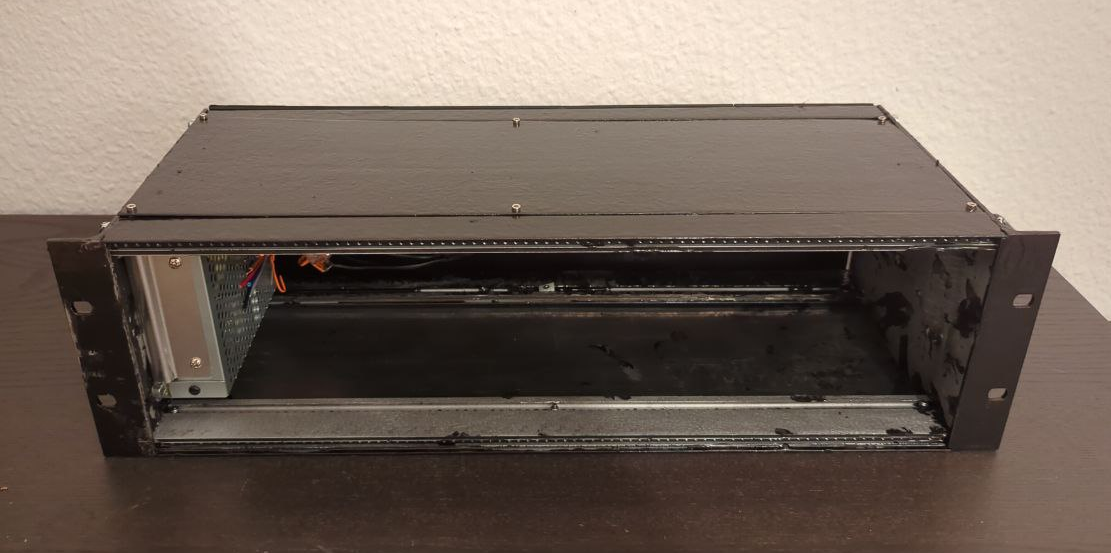
\includegraphics[width=1 \linewidth]{Images/baugruppentraeger1.png}
    \caption{Baugruppenträger mit Netzteil}
    \label{fig:baugruppentraeger}
\end{figure}

\subsection*{Stromverteilung}
Um die Betriebsspannungen für die einzelnen Module verfügbar zu machen, wird eine Platine mit den nötigen IDC-16 Buchsen auf Lochrastermaterial aufgebaut.
Diese verfügt über 8 IDC-16 Buchsen und 4 Schraubterminals zur Verbindung mit dem Netzteil.
Die Platine wird mit 8 3D-Druck-Abstandshaltern (\texttt{./3d/abstandshalter-platinenmontage}) verschraubt, diese wurden mit Epoxidharzkleber an der Rückseite des Gehäuses befestigt.
Die Pinbelegung der IDC-16 Buchse ist der Grafik in Abbildunge \ref{fig:idc16} zu entnehmen. Die Signale Gate und CV sind nicht verbunden.

\begin{figure}[h]
    \centering
    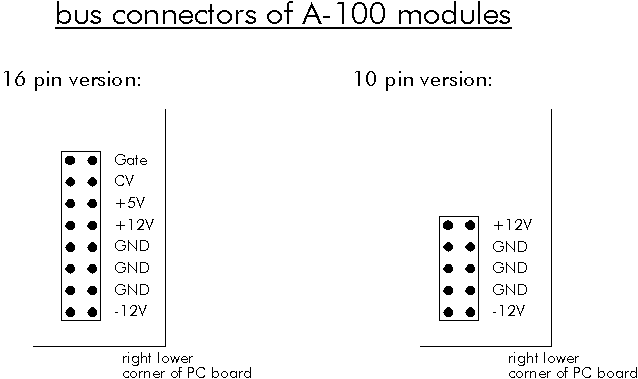
\includegraphics[width= 0.7\linewidth]{Images/idc16.png}
    \caption[Pinbelegung der IDC-16 Buchsen]{Pinbelegung der IDC-16 Buchsen (links)}
    \label{fig:idc16}
\end{figure}
Die entsprechenden Anschlüsse des Netzteils sind mit den Schraubklemmen der Stromversorgungsplatine zu verbinden.

\section{MIDI-Interface}
Die Platine des MIDI-Interfaces wurde in Kicad entworfen und zur Fertigung in Auftrag gegeben.
Die zur Montage benötigten Bauteile sind im Unterverzeichnis \texttt{./doku/Bauteillisten/} zu finden.
Das Platinenlayout ist in Abbildung (\ref{fig:midi-platine}) abgebildet, der Schaltplan in Abbildung \ref{fig:midi-schaltplan}.
\begin{figure}[h]
    \centering
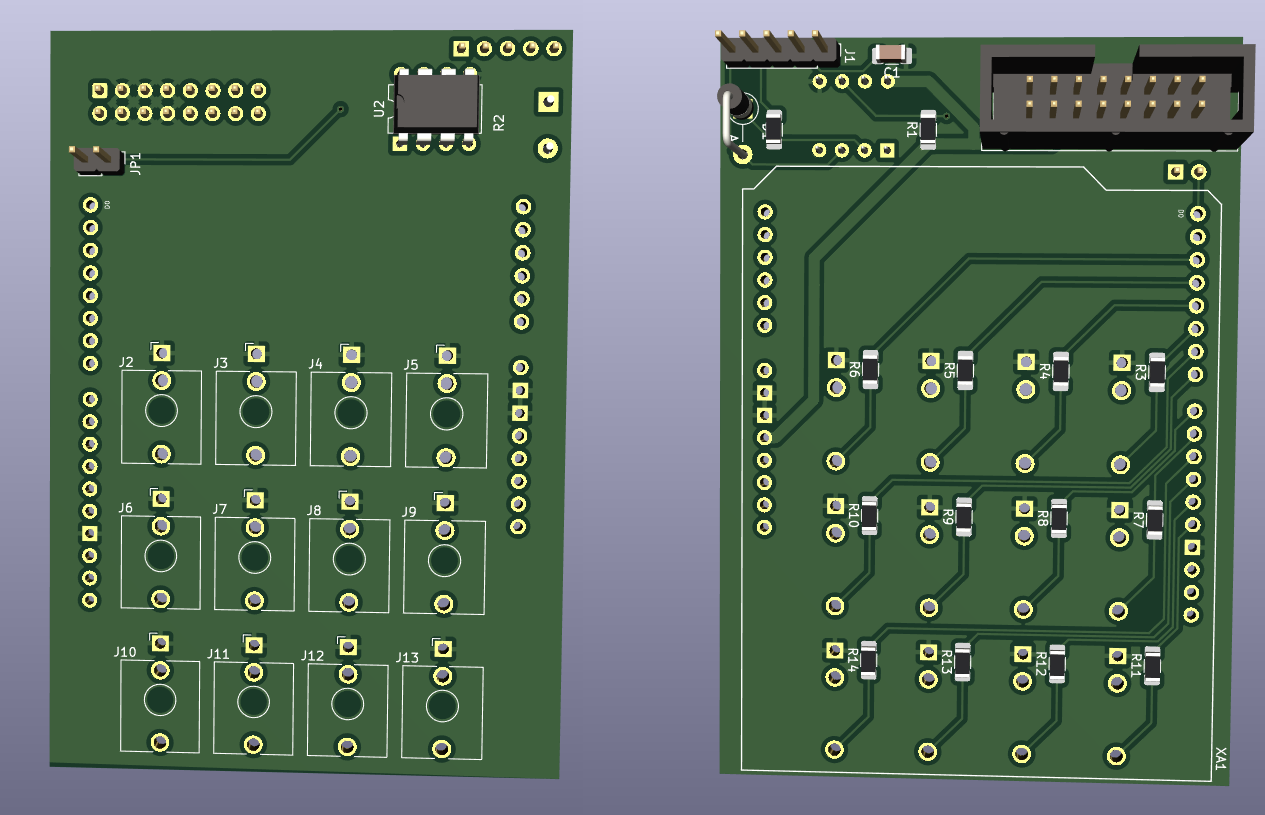
\includegraphics[width=0.7\textwidth]{Images/midi-interface-geschnitten.png}
    \caption{Platinenlayout der MIDI-Platine}
    \label{fig:midi-platine}
\end{figure}
\begin{figure}[h]
    \centering
    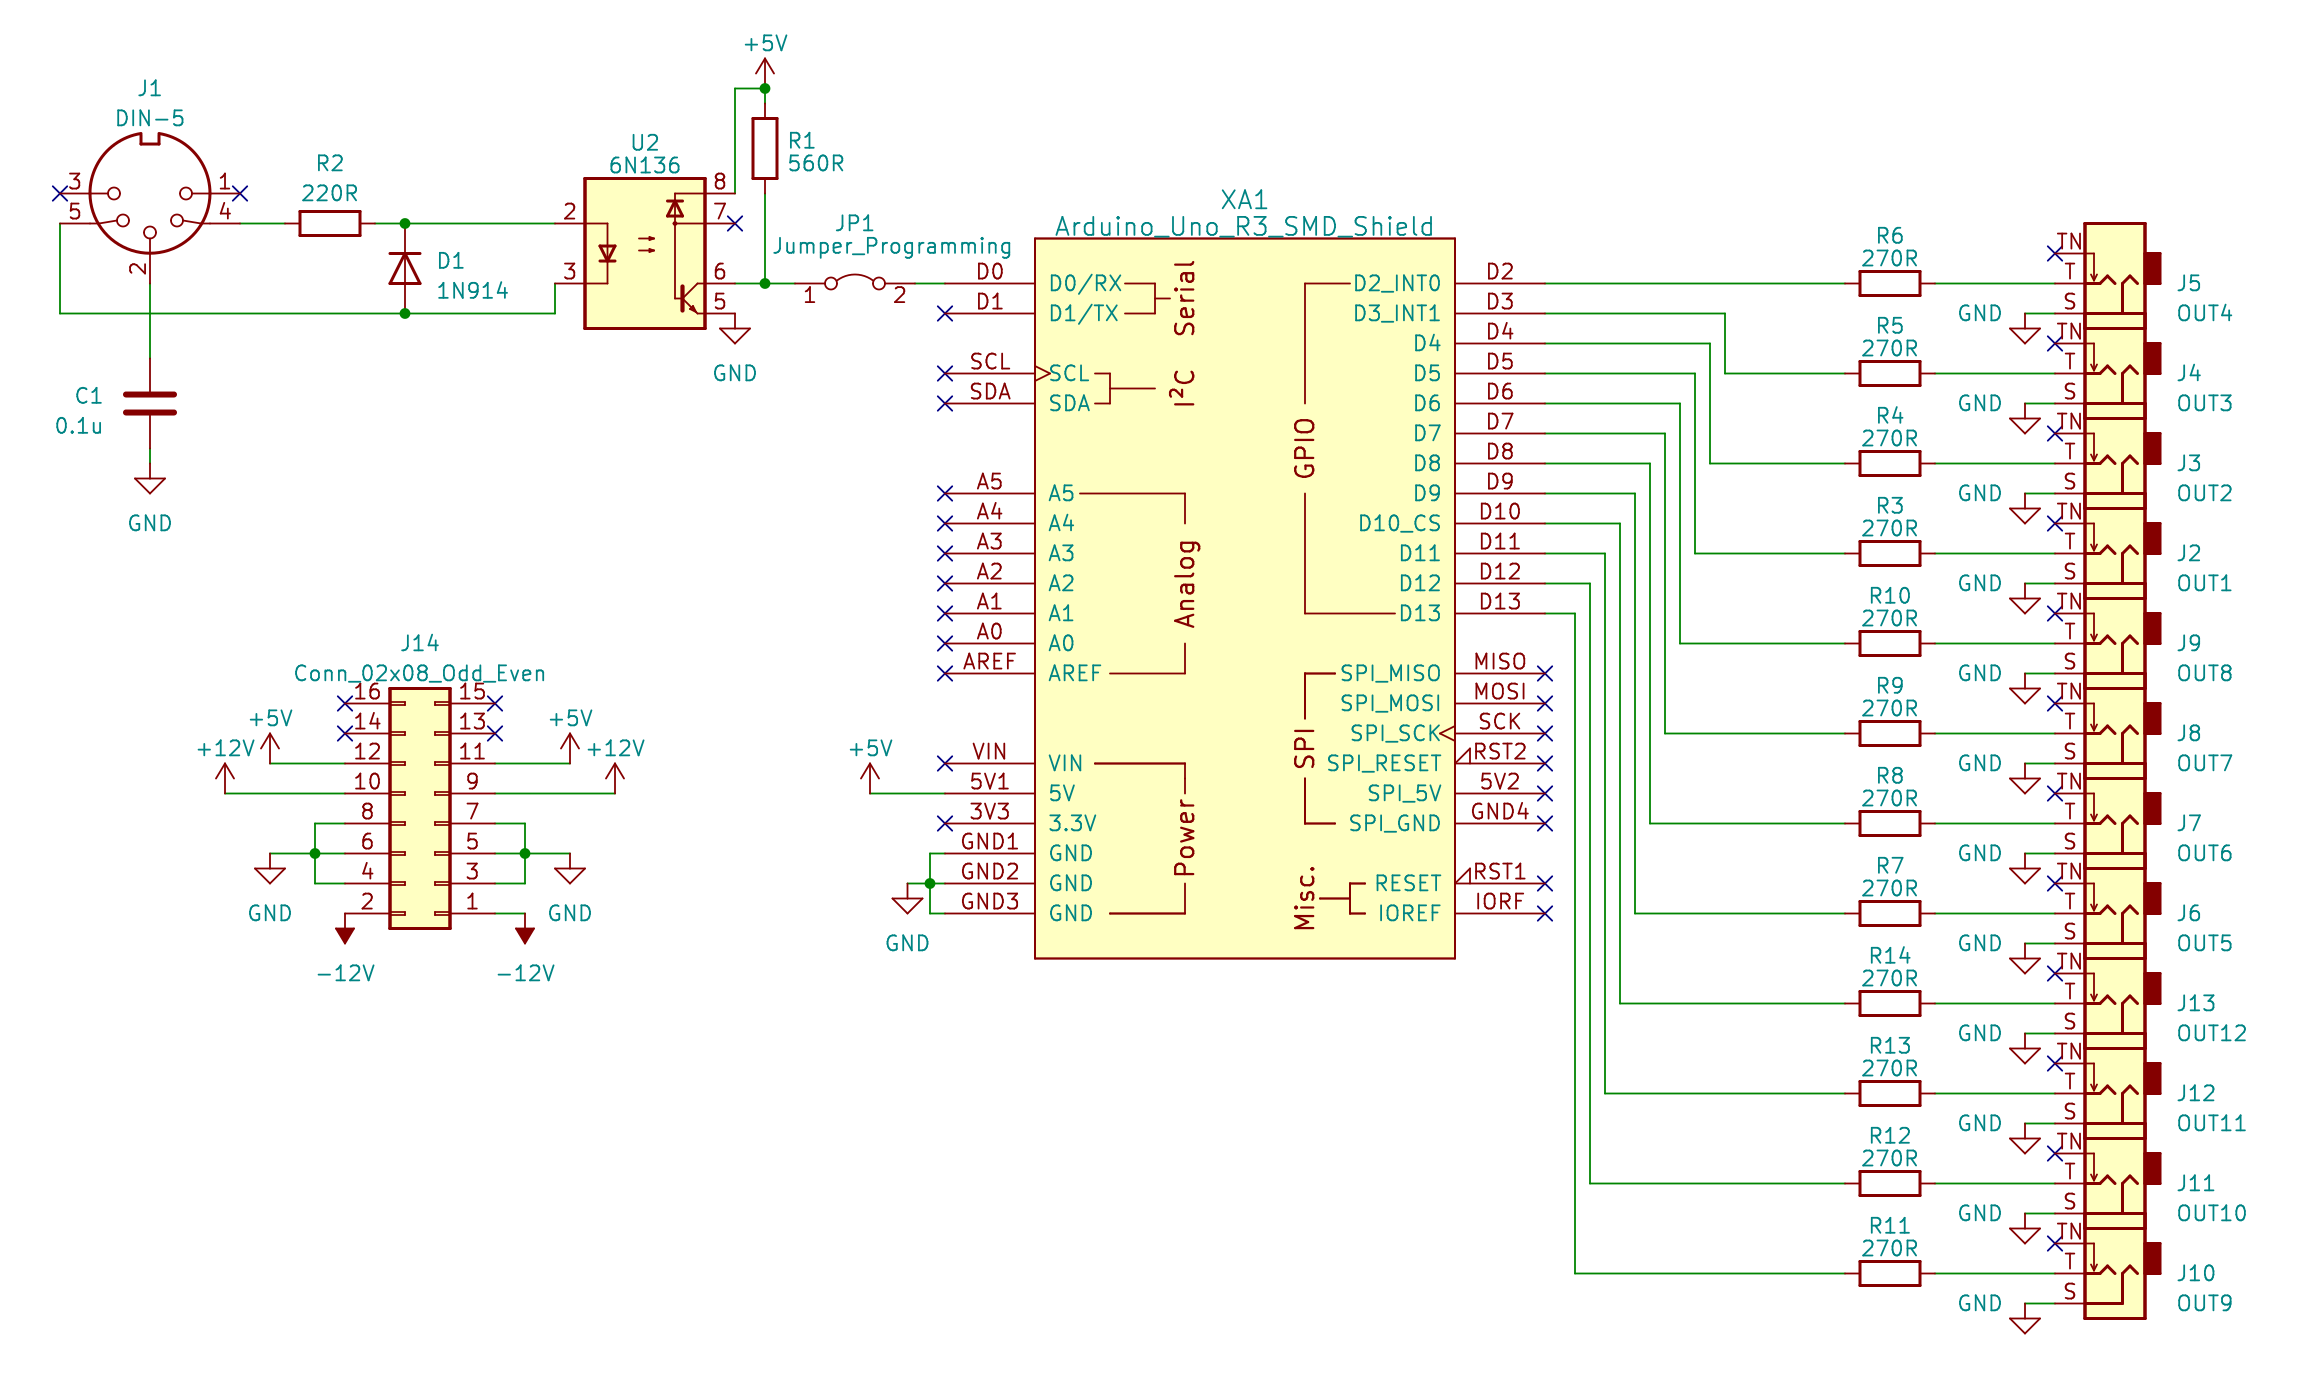
\includegraphics[width=\linewidth]{Images/midi-interface-schematic.png}
    \caption{Schaltplan der MIDI-Interface-Platine}
    \label{fig:midi-schaltplan}
\end{figure}

Nach Auflöten der Bauteile muss der Mikrocontroller programmiert werden.
Der Quellcode ist im Verzeichnis \texttt{./src/midi-interface} zu finden.
Mit dem Befehl \texttt{make \&\& make flash} wird der über USB angeschlossene Arduino programmiert. Dazu werden die Programme make, avrdude und avr-gcc benötigt.

Zur Montage der MIDI-Platine wird eine Frontplatte mit dem 3D-Drucker gefertigt.
Diese ist im Verzeichnis \texttt{./3d/midi/} zu finden.
Die Datei \texttt{frontplatte-midi\_text.scad} beeinhaltet eine alternative Version mit beschrifteten Ausgängen. 
Um die Schrift drucken zu können, muss das Filament nach 3 mm Druckhöhe gegen ein andersfarbiges getauscht werden. 
In der Praxis stellte sich der so aufgedruckte Text als wenig widerstandsfähig heraus, weshalb die Beschriftung der Frontplatte mit einem Labeldrucker geschah.

Die Frontplatte kann nun mit den Muttern der Klinkenbuchse mit der Platine verschraubt werden. Das Modul kann mit 4 M2.5 Schrauben an der Vorderseite des Baugruppenträgers verschraubt werden und mit einem Flachbandkabel mit der Stromversorgung verbunden werden.

\section{Klangerzeuger}
Der Aufbau der Klangerzeugung erfordert eine detaillierte Herangehensweise. Insgesamt stehen 10 verschiedene Klänge zur Verfügung, von denen jede ihre eigene individuelle Schaltung aufweist. Eine Analyse zeigte jedoch, dass diese 10 Klänge auf 3 verschiedene Schaltungstypen zurückgeführt werden können. Aus Kostengründen wurden diese 3 Schaltungstypen auf einer Platine zusammengefasst. Diese ist im Ordner \texttt{./kicad/drummodul} zu finden.

Die Bauteilwerte für die einzelnen Platinen sind in der \enquote{Bauteilliste Klänge} im Ordner \\ \texttt{./doku/Bauteillisten} zu finden.

Anmerkungen: In einigen Klängen, darunter Bassdrum, High Bongo, High Conga, Low Conga, Cymbal 1, Cymbal 2, Maracas und Snaredrum Noise, muss eine Drahtbrücke von C7 zu C9  gelegt werden, um Teile der Schaltung zu überbrücken. Im folgenden Foto sieht man welche Stellen das sind. Die Rote Linie ist die Drahtbrücke

\begin{figure}[H]
    \centering
    \includegraphics[width=0.8\textwidth]{Images/Drahtbrücke.png}
    \caption[Drahtbrücke]{Drahtbrücke}
    \label{fig:Drahtbrücke}
\end{figure}

Je nach Modul werden Frontplatten mit 2 oder 3 Potis benötigt. Diese sind in OpenSCAD entworfen und liegen im Ordner \texttt{./3d/frontplatte-2-potis} bzw. \texttt{./3d/drontplate-3-potis}.

Potentiometer, Taster, Input und Output werden an der Frontplatte angebracht und nicht auf der Platine gelötet. Für die Verbindung stehen 2-polige Stecker vom Typ JST-XH zur Verfügung, die auf die Platine gelötet und dann per Kabel mit den Potentiometern, Tastern und Klinkenbuchsen verbunden werden.
Die Winkel zur Montage der Platine an die Frontplatten liegen in \texttt{./3d/winkel}.
Die Frontplatten werden mit je 2 M2.5x10 Zylinderkopfschrauben und passenden Muttern an den Winkeln befestigt, die Montage der Platine an den Winkeln erfolgt ebenfalls mit 2 M2,5x10 Schrauben.

Ein vollständig montiertes Modul mit Frontplatte ist im folgenden Bild zu erkennen:
\begin{figure}[H]
    \centering
    \includegraphics[width=0.8\textwidth]{Images/modul-aufbau.jpg}
    \caption[Zusammengebautes Modul]{Zusammengebautes Modul}
    \label{fig:Zusammengebautes Modul}
\end{figure}
\section{Summierer und Line-Out}
Um die einzelnen Signale der Klangerzeuger zu Mischen und den Eurorackpegel einem überlichen Line-Out Pegel anzupassen wurden zwei weitere Module angefertigt.
Die Module basieren auf einem invertierenden Summierverstärker bzw. einem invertierenden Verstärker.
Die Schaltpläne dazu sind in \texttt{kicad/line-out} und \texttt{kicad/summierer} zu finden.
Der Platinenaufbau erfolgt auf Lochrasterplatinen.
Die dazugehörigen Frontplatten sind in \texttt{./3d/summierer} und \texttt{./3d/line-out} zu finden. Die Montage erfolgt mit den Winkeln aus \texttt{./3d/winkel}
